% Options for packages loaded elsewhere
\PassOptionsToPackage{unicode}{hyperref}
\PassOptionsToPackage{hyphens}{url}
\PassOptionsToPackage{dvipsnames,svgnames,x11names}{xcolor}
%
\documentclass[
]{article}
\usepackage{amsmath,amssymb}
\usepackage{iftex}
\ifPDFTeX
  \usepackage[T1]{fontenc}
  \usepackage[utf8]{inputenc}
  \usepackage{textcomp} % provide euro and other symbols
\else % if luatex or xetex
  \usepackage{unicode-math} % this also loads fontspec
  \defaultfontfeatures{Scale=MatchLowercase}
  \defaultfontfeatures[\rmfamily]{Ligatures=TeX,Scale=1}
\fi
\usepackage{lmodern}
\ifPDFTeX\else
  % xetex/luatex font selection
\fi
% Use upquote if available, for straight quotes in verbatim environments
\IfFileExists{upquote.sty}{\usepackage{upquote}}{}
\IfFileExists{microtype.sty}{% use microtype if available
  \usepackage[]{microtype}
  \UseMicrotypeSet[protrusion]{basicmath} % disable protrusion for tt fonts
}{}
\makeatletter
\@ifundefined{KOMAClassName}{% if non-KOMA class
  \IfFileExists{parskip.sty}{%
    \usepackage{parskip}
  }{% else
    \setlength{\parindent}{0pt}
    \setlength{\parskip}{6pt plus 2pt minus 1pt}}
}{% if KOMA class
  \KOMAoptions{parskip=half}}
\makeatother
\usepackage{xcolor}
\usepackage[margin=1in]{geometry}
\usepackage{color}
\usepackage{fancyvrb}
\newcommand{\VerbBar}{|}
\newcommand{\VERB}{\Verb[commandchars=\\\{\}]}
\DefineVerbatimEnvironment{Highlighting}{Verbatim}{commandchars=\\\{\}}
% Add ',fontsize=\small' for more characters per line
\usepackage{framed}
\definecolor{shadecolor}{RGB}{248,248,248}
\newenvironment{Shaded}{\begin{snugshade}}{\end{snugshade}}
\newcommand{\AlertTok}[1]{\textcolor[rgb]{0.94,0.16,0.16}{#1}}
\newcommand{\AnnotationTok}[1]{\textcolor[rgb]{0.56,0.35,0.01}{\textbf{\textit{#1}}}}
\newcommand{\AttributeTok}[1]{\textcolor[rgb]{0.13,0.29,0.53}{#1}}
\newcommand{\BaseNTok}[1]{\textcolor[rgb]{0.00,0.00,0.81}{#1}}
\newcommand{\BuiltInTok}[1]{#1}
\newcommand{\CharTok}[1]{\textcolor[rgb]{0.31,0.60,0.02}{#1}}
\newcommand{\CommentTok}[1]{\textcolor[rgb]{0.56,0.35,0.01}{\textit{#1}}}
\newcommand{\CommentVarTok}[1]{\textcolor[rgb]{0.56,0.35,0.01}{\textbf{\textit{#1}}}}
\newcommand{\ConstantTok}[1]{\textcolor[rgb]{0.56,0.35,0.01}{#1}}
\newcommand{\ControlFlowTok}[1]{\textcolor[rgb]{0.13,0.29,0.53}{\textbf{#1}}}
\newcommand{\DataTypeTok}[1]{\textcolor[rgb]{0.13,0.29,0.53}{#1}}
\newcommand{\DecValTok}[1]{\textcolor[rgb]{0.00,0.00,0.81}{#1}}
\newcommand{\DocumentationTok}[1]{\textcolor[rgb]{0.56,0.35,0.01}{\textbf{\textit{#1}}}}
\newcommand{\ErrorTok}[1]{\textcolor[rgb]{0.64,0.00,0.00}{\textbf{#1}}}
\newcommand{\ExtensionTok}[1]{#1}
\newcommand{\FloatTok}[1]{\textcolor[rgb]{0.00,0.00,0.81}{#1}}
\newcommand{\FunctionTok}[1]{\textcolor[rgb]{0.13,0.29,0.53}{\textbf{#1}}}
\newcommand{\ImportTok}[1]{#1}
\newcommand{\InformationTok}[1]{\textcolor[rgb]{0.56,0.35,0.01}{\textbf{\textit{#1}}}}
\newcommand{\KeywordTok}[1]{\textcolor[rgb]{0.13,0.29,0.53}{\textbf{#1}}}
\newcommand{\NormalTok}[1]{#1}
\newcommand{\OperatorTok}[1]{\textcolor[rgb]{0.81,0.36,0.00}{\textbf{#1}}}
\newcommand{\OtherTok}[1]{\textcolor[rgb]{0.56,0.35,0.01}{#1}}
\newcommand{\PreprocessorTok}[1]{\textcolor[rgb]{0.56,0.35,0.01}{\textit{#1}}}
\newcommand{\RegionMarkerTok}[1]{#1}
\newcommand{\SpecialCharTok}[1]{\textcolor[rgb]{0.81,0.36,0.00}{\textbf{#1}}}
\newcommand{\SpecialStringTok}[1]{\textcolor[rgb]{0.31,0.60,0.02}{#1}}
\newcommand{\StringTok}[1]{\textcolor[rgb]{0.31,0.60,0.02}{#1}}
\newcommand{\VariableTok}[1]{\textcolor[rgb]{0.00,0.00,0.00}{#1}}
\newcommand{\VerbatimStringTok}[1]{\textcolor[rgb]{0.31,0.60,0.02}{#1}}
\newcommand{\WarningTok}[1]{\textcolor[rgb]{0.56,0.35,0.01}{\textbf{\textit{#1}}}}
\usepackage{graphicx}
\makeatletter
\def\maxwidth{\ifdim\Gin@nat@width>\linewidth\linewidth\else\Gin@nat@width\fi}
\def\maxheight{\ifdim\Gin@nat@height>\textheight\textheight\else\Gin@nat@height\fi}
\makeatother
% Scale images if necessary, so that they will not overflow the page
% margins by default, and it is still possible to overwrite the defaults
% using explicit options in \includegraphics[width, height, ...]{}
\setkeys{Gin}{width=\maxwidth,height=\maxheight,keepaspectratio}
% Set default figure placement to htbp
\makeatletter
\def\fps@figure{htbp}
\makeatother
\setlength{\emergencystretch}{3em} % prevent overfull lines
\providecommand{\tightlist}{%
  \setlength{\itemsep}{0pt}\setlength{\parskip}{0pt}}
\setcounter{secnumdepth}{-\maxdimen} % remove section numbering
\ifLuaTeX
  \usepackage{selnolig}  % disable illegal ligatures
\fi
\usepackage{bookmark}
\IfFileExists{xurl.sty}{\usepackage{xurl}}{} % add URL line breaks if available
\urlstyle{same}
\hypersetup{
  pdftitle={Module 7: Solutions to recommended Exercises},
  pdfauthor={Sara Martino, Stefanie Muff, Kenneth Aase; Department of Mathematical Sciences, NTNU},
  colorlinks=true,
  linkcolor={Maroon},
  filecolor={Maroon},
  citecolor={Blue},
  urlcolor={blue},
  pdfcreator={LaTeX via pandoc}}

\title{Module 7: Solutions to recommended Exercises}
\usepackage{etoolbox}
\makeatletter
\providecommand{\subtitle}[1]{% add subtitle to \maketitle
  \apptocmd{\@title}{\par {\large #1 \par}}{}{}
}
\makeatother
\subtitle{TMA4268 Statistical Learning V2025}
\author{Sara Martino, Stefanie Muff, Kenneth Aase \and Department of
Mathematical Sciences, NTNU}
\date{Feb 28, 2025}

\begin{document}
\maketitle

\subsection{Problem 1}\label{problem-1}

The code below performs polynomial regression of degree \(1\), \(2\),
\(3\) and \(4\). The function \texttt{sapply()} is an efficient
for-loop. We iterate over all degrees to plot the fitted values and
compute the test error. Finally we plot the test error for each
polynomial degree.

\begin{Shaded}
\begin{Highlighting}[]
\FunctionTok{library}\NormalTok{(ISLR)}
\CommentTok{\# extract only the two variables from Auto}
\NormalTok{ds }\OtherTok{\textless{}{-}}\NormalTok{ Auto[}\FunctionTok{c}\NormalTok{(}\StringTok{"horsepower"}\NormalTok{, }\StringTok{"mpg"}\NormalTok{)]}
\NormalTok{n }\OtherTok{\textless{}{-}} \FunctionTok{nrow}\NormalTok{(ds)}
\CommentTok{\# which degrees we will look at}
\NormalTok{deg }\OtherTok{\textless{}{-}} \DecValTok{1}\SpecialCharTok{:}\DecValTok{4}
\FunctionTok{set.seed}\NormalTok{(}\DecValTok{1}\NormalTok{)}
\CommentTok{\# training ids for training set}
\NormalTok{tr }\OtherTok{\textless{}{-}} \FunctionTok{sample.int}\NormalTok{(n, n }\SpecialCharTok{/} \DecValTok{2}\NormalTok{)}
\CommentTok{\# plot of training data}
\FunctionTok{plot}\NormalTok{(ds[tr, ], }\AttributeTok{col =} \StringTok{"darkgrey"}\NormalTok{, }\AttributeTok{main =} \StringTok{"Polynomial regression"}\NormalTok{)}

\CommentTok{\# which colors we will plot the lines with}
\NormalTok{co }\OtherTok{\textless{}{-}} \FunctionTok{rainbow}\NormalTok{(}\FunctionTok{length}\NormalTok{(deg))}
\CommentTok{\# iterate over all degrees (1:4) {-} could also use a for{-}loop here}
\NormalTok{MSE }\OtherTok{\textless{}{-}} \FunctionTok{sapply}\NormalTok{(deg, }\ControlFlowTok{function}\NormalTok{(d) \{}
  \CommentTok{\# fit model with this degree}
\NormalTok{  mod }\OtherTok{\textless{}{-}} \FunctionTok{lm}\NormalTok{(mpg }\SpecialCharTok{\textasciitilde{}} \FunctionTok{poly}\NormalTok{(horsepower, d), ds[tr, ])}
  \CommentTok{\# add lines to the plot }
  \CommentTok{\# use fitted values (for mpg) and horsepower from training set}
  \FunctionTok{lines}\NormalTok{(}\FunctionTok{cbind}\NormalTok{(ds[tr, }\DecValTok{1}\NormalTok{], mod}\SpecialCharTok{$}\NormalTok{fit)[}\FunctionTok{order}\NormalTok{(ds[tr, }\DecValTok{1}\NormalTok{]), ], }\AttributeTok{col =}\NormalTok{ co[d])}
  \CommentTok{\# calculate mean MSE {-} this is returned in the MSE variable}
  \FunctionTok{mean}\NormalTok{((}\FunctionTok{predict}\NormalTok{(mod, ds[}\SpecialCharTok{{-}}\NormalTok{tr, ]) }\SpecialCharTok{{-}}\NormalTok{ ds[}\SpecialCharTok{{-}}\NormalTok{tr, }\DecValTok{2}\NormalTok{])}\SpecialCharTok{\^{}}\DecValTok{2}\NormalTok{)}
\NormalTok{\})}
\CommentTok{\# add legend to see which color corresponds to which line}
\FunctionTok{legend}\NormalTok{(}\StringTok{"topright"}\NormalTok{, }\AttributeTok{legend =} \FunctionTok{paste}\NormalTok{(}\StringTok{"d ="}\NormalTok{, deg), }\AttributeTok{lty =} \DecValTok{1}\NormalTok{, }\AttributeTok{col =}\NormalTok{ co)}
\end{Highlighting}
\end{Shaded}

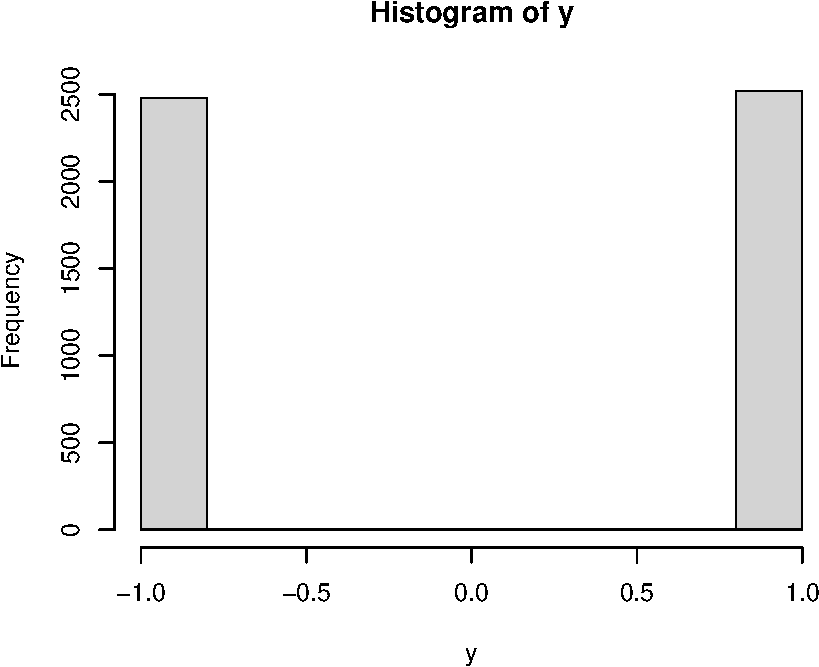
\includegraphics{RecEx7-sol_files/figure-latex/unnamed-chunk-1-1.pdf}

\begin{Shaded}
\begin{Highlighting}[]
\CommentTok{\# plot MSE}
\FunctionTok{plot}\NormalTok{(MSE, }\AttributeTok{type =} \StringTok{"o"}\NormalTok{, }\AttributeTok{pch =} \DecValTok{16}\NormalTok{, }\AttributeTok{xlab =} \StringTok{"degree"}\NormalTok{, }\AttributeTok{main =} \StringTok{"Test error"}\NormalTok{)}
\end{Highlighting}
\end{Shaded}

\includegraphics{RecEx7-sol_files/figure-latex/unnamed-chunk-1-2.pdf}

The same solution using \texttt{ggplot} is shown below.

\begin{Shaded}
\begin{Highlighting}[]
\CommentTok{\# solution with ggplot}
\FunctionTok{library}\NormalTok{(ISLR)}
\FunctionTok{library}\NormalTok{(ggplot2)}
\CommentTok{\# extract only the two variables from Auto}
\NormalTok{ds }\OtherTok{\textless{}{-}}\NormalTok{ Auto[}\FunctionTok{c}\NormalTok{(}\StringTok{"horsepower"}\NormalTok{, }\StringTok{"mpg"}\NormalTok{)]}
\NormalTok{n }\OtherTok{\textless{}{-}} \FunctionTok{nrow}\NormalTok{(ds)}
\CommentTok{\# which degrees we will look at}
\NormalTok{deg }\OtherTok{\textless{}{-}} \DecValTok{1}\SpecialCharTok{:}\DecValTok{4}
\FunctionTok{set.seed}\NormalTok{(}\DecValTok{1}\NormalTok{)}
\CommentTok{\# training ids for training set}
\NormalTok{tr }\OtherTok{\textless{}{-}} \FunctionTok{sample.int}\NormalTok{(n, n }\SpecialCharTok{/} \DecValTok{2}\NormalTok{)}
\CommentTok{\# plot of training data}
\FunctionTok{ggplot}\NormalTok{(}\AttributeTok{data =}\NormalTok{ ds[tr, ], }\FunctionTok{aes}\NormalTok{(}\AttributeTok{x =}\NormalTok{ horsepower, }\AttributeTok{y =}\NormalTok{ mpg)) }\SpecialCharTok{+}
  \FunctionTok{geom\_point}\NormalTok{(}\AttributeTok{color =} \StringTok{"darkgrey"}\NormalTok{) }\SpecialCharTok{+}
  \FunctionTok{labs}\NormalTok{(}\AttributeTok{title =} \StringTok{"Polynomial regression"}\NormalTok{)}
\end{Highlighting}
\end{Shaded}

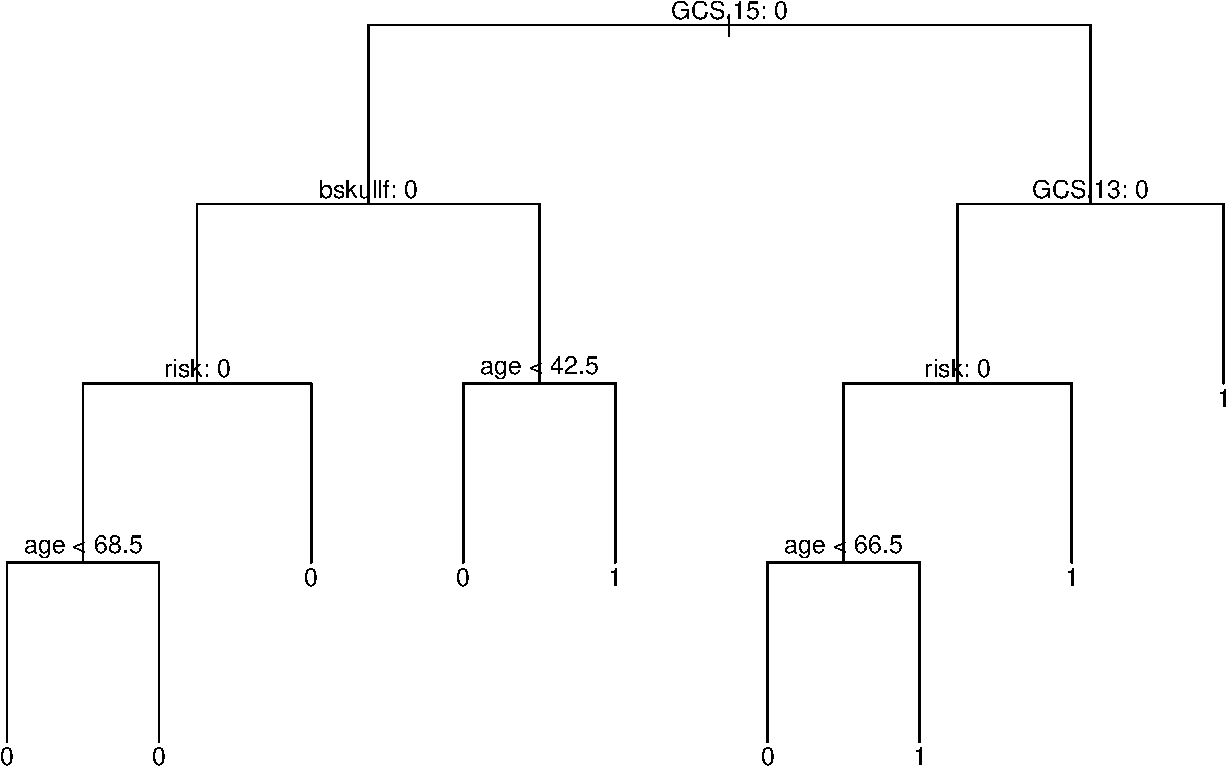
\includegraphics{RecEx7-sol_files/figure-latex/unnamed-chunk-2-1.pdf}

\begin{Shaded}
\begin{Highlighting}[]
\CommentTok{\# iterate over all degrees (1:4) {-} could also use a for{-}loop here}
\NormalTok{dat }\OtherTok{\textless{}{-}} \FunctionTok{c}\NormalTok{() }\CommentTok{\# make a empty variable to store predicted values}
\ControlFlowTok{for}\NormalTok{ (d }\ControlFlowTok{in}\NormalTok{ deg) \{}
  \CommentTok{\# fit model with this degree}
\NormalTok{  mod }\OtherTok{\textless{}{-}} \FunctionTok{lm}\NormalTok{(mpg }\SpecialCharTok{\textasciitilde{}} \FunctionTok{poly}\NormalTok{(horsepower, d), ds[tr, ])}
  \CommentTok{\# data frame of predicted values {-} use fitted values (for mpg) and horsepower }
  \CommentTok{\# from training set and add column (factor) for degree}
\NormalTok{  dat }\OtherTok{\textless{}{-}} \FunctionTok{rbind}\NormalTok{(dat, }\FunctionTok{data.frame}\NormalTok{(}
    \AttributeTok{horsepower =}\NormalTok{ ds[tr, }\DecValTok{1}\NormalTok{], }\AttributeTok{mpg =}\NormalTok{ mod}\SpecialCharTok{$}\NormalTok{fit,}
    \AttributeTok{degree =} \FunctionTok{as.factor}\NormalTok{(}\FunctionTok{rep}\NormalTok{(d, }\FunctionTok{length}\NormalTok{(mod}\SpecialCharTok{$}\NormalTok{fit)))}
\NormalTok{  ))}
  \CommentTok{\# calculate mean MSE {-} this is returned in the MSE variable}
\NormalTok{  MSE[d] }\OtherTok{\textless{}{-}} \FunctionTok{mean}\NormalTok{((}\FunctionTok{predict}\NormalTok{(mod, ds[}\SpecialCharTok{{-}}\NormalTok{tr, ]) }\SpecialCharTok{{-}}\NormalTok{ ds[}\SpecialCharTok{{-}}\NormalTok{tr, }\DecValTok{2}\NormalTok{])}\SpecialCharTok{\^{}}\DecValTok{2}\NormalTok{)}
\NormalTok{\}}
\CommentTok{\# plot fitted values for different degrees}
\FunctionTok{ggplot}\NormalTok{(}\AttributeTok{data =}\NormalTok{ ds[tr, ], }\FunctionTok{aes}\NormalTok{(}\AttributeTok{x =}\NormalTok{ horsepower, }\AttributeTok{y =}\NormalTok{ mpg)) }\SpecialCharTok{+}
  \FunctionTok{geom\_point}\NormalTok{(}\AttributeTok{color =} \StringTok{"darkgrey"}\NormalTok{) }\SpecialCharTok{+}
  \FunctionTok{labs}\NormalTok{(}\AttributeTok{title =} \StringTok{"Polynomial regression"}\NormalTok{) }\SpecialCharTok{+}
  \FunctionTok{geom\_line}\NormalTok{(}\AttributeTok{data =}\NormalTok{ dat, }\FunctionTok{aes}\NormalTok{(}\AttributeTok{x =}\NormalTok{ horsepower, }\AttributeTok{y =}\NormalTok{ mpg, }\AttributeTok{color =}\NormalTok{ degree))}
\end{Highlighting}
\end{Shaded}

\includegraphics{RecEx7-sol_files/figure-latex/unnamed-chunk-2-2.pdf}

\begin{Shaded}
\begin{Highlighting}[]
\CommentTok{\# plot MSE}
\NormalTok{MSEdata }\OtherTok{\textless{}{-}} \FunctionTok{data.frame}\NormalTok{(}\AttributeTok{MSE =}\NormalTok{ MSE, }\AttributeTok{degree =} \DecValTok{1}\SpecialCharTok{:}\DecValTok{4}\NormalTok{)}
\FunctionTok{ggplot}\NormalTok{(}\AttributeTok{data =}\NormalTok{ MSEdata, }\FunctionTok{aes}\NormalTok{(}\AttributeTok{x =}\NormalTok{ degree, }\AttributeTok{y =}\NormalTok{ MSE)) }\SpecialCharTok{+}
  \FunctionTok{geom\_line}\NormalTok{() }\SpecialCharTok{+}
  \FunctionTok{geom\_point}\NormalTok{() }\SpecialCharTok{+}
  \FunctionTok{labs}\NormalTok{(}\AttributeTok{title =} \StringTok{"Test error"}\NormalTok{)}
\end{Highlighting}
\end{Shaded}

\includegraphics{RecEx7-sol_files/figure-latex/unnamed-chunk-2-3.pdf}

\subsection{Problem 2}\label{problem-2}

We use \texttt{factor(origin)} for conversion to a factor variable. The
function \texttt{predict(...,\ se\ =\ TRUE)} gives fitted values with
standard errors.

\begin{Shaded}
\begin{Highlighting}[]
\FunctionTok{attach}\NormalTok{(Auto)}
\CommentTok{\# fit model}
\NormalTok{fit }\OtherTok{\textless{}{-}} \FunctionTok{lm}\NormalTok{(mpg }\SpecialCharTok{\textasciitilde{}} \FunctionTok{factor}\NormalTok{(origin))}
\CommentTok{\# make a new dataset of the origins to predict the mpg for the different origins}
\NormalTok{new }\OtherTok{\textless{}{-}} \FunctionTok{data.frame}\NormalTok{(}\AttributeTok{origin =} \FunctionTok{as.factor}\NormalTok{(}\FunctionTok{sort}\NormalTok{(}\FunctionTok{unique}\NormalTok{(origin))))}
\CommentTok{\# predicted values and standard errors}
\NormalTok{pred }\OtherTok{\textless{}{-}} \FunctionTok{predict}\NormalTok{(fit, new, }\AttributeTok{se =} \ConstantTok{TRUE}\NormalTok{)}
\CommentTok{\# data frame including CI (z\_alpha/2 = 1.96)}
\NormalTok{dat }\OtherTok{\textless{}{-}} \FunctionTok{data.frame}\NormalTok{(}
  \AttributeTok{origin =}\NormalTok{ new, }\AttributeTok{mpg =}\NormalTok{ pred}\SpecialCharTok{$}\NormalTok{fit,}
  \AttributeTok{lwr =}\NormalTok{ pred}\SpecialCharTok{$}\NormalTok{fit }\SpecialCharTok{{-}} \FloatTok{1.96} \SpecialCharTok{*}\NormalTok{ pred}\SpecialCharTok{$}\NormalTok{se.fit,}
  \AttributeTok{upr =}\NormalTok{ pred}\SpecialCharTok{$}\NormalTok{fit }\SpecialCharTok{+} \FloatTok{1.96} \SpecialCharTok{*}\NormalTok{ pred}\SpecialCharTok{$}\NormalTok{se.fit)}

\CommentTok{\# plot the fitted/predicted values and CI}
\FunctionTok{ggplot}\NormalTok{(dat, }\FunctionTok{aes}\NormalTok{(}\AttributeTok{x =}\NormalTok{ origin, }\AttributeTok{y =}\NormalTok{ mpg)) }\SpecialCharTok{+}
  \FunctionTok{geom\_point}\NormalTok{() }\SpecialCharTok{+}
  \FunctionTok{geom\_segment}\NormalTok{(}\FunctionTok{aes}\NormalTok{(}\AttributeTok{x =}\NormalTok{ origin, }\AttributeTok{y =}\NormalTok{ lwr, }\AttributeTok{xend =}\NormalTok{ origin, }\AttributeTok{yend =}\NormalTok{ upr)) }\SpecialCharTok{+}
  \FunctionTok{scale\_x\_discrete}\NormalTok{(}\AttributeTok{labels =} \FunctionTok{c}\NormalTok{(}\StringTok{"1"} \OtherTok{=} \StringTok{"1.American"}\NormalTok{,}
                              \StringTok{"2"} \OtherTok{=} \StringTok{"2.European"}\NormalTok{,}
                              \StringTok{"3"} \OtherTok{=} \StringTok{"3.Japanese"}\NormalTok{))}
\end{Highlighting}
\end{Shaded}

\includegraphics{RecEx7-sol_files/figure-latex/unnamed-chunk-3-1.pdf}

\subsection{Problem 3}\label{problem-3}

The request is a design matrix \(X\) for a natural cubic spline with
\(X =\) \texttt{year} and one internal knot at \(2006\). The definition
of the basis for a natural cubic spline is \[
b_1(x_i) = x_i, \quad b_{k+2}(x_i) = d_k(x_i)-d_K(x_i),\; k = 0, \ldots, K - 1,\\
\]

\[
d_k(x_i) = \frac{(x_i-c_k)^3_+-(x_i-c_{K+1})^3_+}{c_{K+1}-c_k},
\]

where \(K\) is the number of internal knots, \(c_k\) is the location of
the \(k^\text{th}\) knot, and \((.)_+\) denotes \(\max (., 0)\). In our
case we have one internal knot at \(c_1 = 2006\), thus \(K = 1\). Since
this is a natural spline, the boundary knots should be the extreme
values of \texttt{year}, that is \(c_0 = 2003\) and \(c_2 = 2009\).
Since \(K=1\), the index \(k\) takes only the value \(0\), so we end up
with only having to find \(b_1(x_i)\) and \(b_2(x_i)\).

By inserting into the above expressions, we find that the two basis
functions are

\begin{align*}
b_1(x_i) &= x_i,\\
b_2(x_i) &= d_0(x_i)-d_1(x_i)\\
&= \frac{(x_i-c_0)^3_+-(x_i-c_2)^3_+}{c_2-c_0} - \frac{(x_i-c_1)^3_+-(x_i-c_2)^3_+}{c_2-c_1}\\
&= \frac{1}{c_2-c_0}(x_i-c_0)^3_+ - \frac{1}{c_2-c_1}(x_i-c_1)^3_+ + \left(\frac{1}{c_2-c_1}-\frac{1}{c_2-c_0}\right)(x_i-c_{2})^3_+\\
&= \frac{1}{6}(x_i-2003)^3_+ - \frac{1}{3}(x_i-2006)^3_+ + \frac{1}{6}(x_i-2009)^3_+.
\end{align*}

We can simplify the final term in the second basis function by using the
fact that the boundary knots are the extreme values of \(x_i\), that is
\(2003 \leq x_i \leq 2009\), and thus \(\frac{1}{6}(x_i-2009)^3_+=0\).
Thus,

\[
b_2(x_i) = \frac{1}{6}(x_i-2003)^3 - \frac{1}{3}(x_i-2006)^3_+.
\]

The design matrix (here also including an intercept term) is given by

\[
\mathbf X = \begin{pmatrix}
1 & b_{1}(x_1) & b_{2}(x_1) \\
1 & b_{1}(x_2) & b_{2}(x_2) \\
\vdots & \vdots & \vdots \\
1 & b_{1}(x_n) & b_{2}(x_n) \\
\end{pmatrix},
\]

where \(b_1(x_i)\) and \(b_2(x_i)\) are as found above.

\subsection{Problem 4}\label{problem-4}

The matrix \(\mathbf X\) is obtained by using \texttt{cbind()} to join
an intercept, a cubic spline, a natural cubic spline and a factor.

\begin{Shaded}
\begin{Highlighting}[]
\FunctionTok{library}\NormalTok{(ISLR)}
\FunctionTok{attach}\NormalTok{(Wage)}
\CommentTok{\# install.packages("gam")}
\FunctionTok{library}\NormalTok{(gam)}

\CommentTok{\# Write a couple of functions first, which will be used to produce the }
\CommentTok{\# components of the design matrix.}
\CommentTok{\# We write separate functions to generate X\_1, X\_2 and X\_3 (the three components}
\CommentTok{\# of the model)}
\CommentTok{\# X\_1: The function mybs() generates basis functions for the cubic spline}
\NormalTok{mybs }\OtherTok{\textless{}{-}} \ControlFlowTok{function}\NormalTok{(x, knots) \{}
  \FunctionTok{cbind}\NormalTok{(x, x}\SpecialCharTok{\^{}}\DecValTok{2}\NormalTok{, x}\SpecialCharTok{\^{}}\DecValTok{3}\NormalTok{, }\FunctionTok{sapply}\NormalTok{(knots, }\ControlFlowTok{function}\NormalTok{(y) }\FunctionTok{pmax}\NormalTok{(}\DecValTok{0}\NormalTok{, x }\SpecialCharTok{{-}}\NormalTok{ y)}\SpecialCharTok{\^{}}\DecValTok{3}\NormalTok{))}
\NormalTok{\} }

\CommentTok{\# X\_2: The function myns generates basis functions for the natural cubic spline;}
\CommentTok{\# d() is a helper function}
\NormalTok{d }\OtherTok{\textless{}{-}} \ControlFlowTok{function}\NormalTok{(c, cK, x) \{}
\NormalTok{  (}\FunctionTok{pmax}\NormalTok{(}\DecValTok{0}\NormalTok{, x }\SpecialCharTok{{-}}\NormalTok{ c)}\SpecialCharTok{\^{}}\DecValTok{3} \SpecialCharTok{{-}} \FunctionTok{pmax}\NormalTok{(}\DecValTok{0}\NormalTok{, x }\SpecialCharTok{{-}}\NormalTok{ cK)}\SpecialCharTok{\^{}}\DecValTok{3}\NormalTok{) }\SpecialCharTok{/}\NormalTok{ (cK }\SpecialCharTok{{-}}\NormalTok{ c)}
\NormalTok{\}}
\NormalTok{myns }\OtherTok{\textless{}{-}} \ControlFlowTok{function}\NormalTok{(x, knots) \{}
\NormalTok{  kn }\OtherTok{\textless{}{-}} \FunctionTok{c}\NormalTok{(}\FunctionTok{min}\NormalTok{(x), knots, }\FunctionTok{max}\NormalTok{(x))}
\NormalTok{  K }\OtherTok{\textless{}{-}} \FunctionTok{length}\NormalTok{(kn)}
\NormalTok{  sub }\OtherTok{\textless{}{-}} \FunctionTok{d}\NormalTok{(kn[K }\SpecialCharTok{{-}} \DecValTok{1}\NormalTok{], kn[K], x)}
  \FunctionTok{cbind}\NormalTok{(x, }\FunctionTok{sapply}\NormalTok{(kn[}\DecValTok{1}\SpecialCharTok{:}\NormalTok{(K }\SpecialCharTok{{-}} \DecValTok{2}\NormalTok{)], d, kn[K], x) }\SpecialCharTok{{-}}\NormalTok{ sub)}
\NormalTok{\}}

\CommentTok{\# X\_3: The function myfactor() generates the dummy{-}basis functions for a factor}
\CommentTok{\# covariate, building on the R{-}function model.matrix()}
\NormalTok{myfactor }\OtherTok{\textless{}{-}} \ControlFlowTok{function}\NormalTok{(x) \{}
  \FunctionTok{model.matrix}\NormalTok{(}\SpecialCharTok{\textasciitilde{}}\NormalTok{x)[, }\SpecialCharTok{{-}}\DecValTok{1}\NormalTok{]}
\NormalTok{\}}

\CommentTok{\# Once these functions are prepared, we can generate the model matrix}
\CommentTok{\# X = (1,X\_1, X\_2, X\_3) as a one{-}liner}
\NormalTok{X }\OtherTok{\textless{}{-}} \FunctionTok{cbind}\NormalTok{(}\DecValTok{1}\NormalTok{, }\FunctionTok{mybs}\NormalTok{(age, }\FunctionTok{c}\NormalTok{(}\DecValTok{40}\NormalTok{, }\DecValTok{60}\NormalTok{)), }\FunctionTok{myns}\NormalTok{(year, }\DecValTok{2006}\NormalTok{), }\FunctionTok{myfactor}\NormalTok{(education))}
\end{Highlighting}
\end{Shaded}

We have now created a model matrix \(\mathbf X\) ``by hand''. The thing
we wanted to illustrate with this exercise is that this hand-made matrix
does not correspond to the internal representation of the model matrix
that we would direclty get using the \texttt{gam()} function:

\begin{Shaded}
\begin{Highlighting}[]
\NormalTok{X\_gam }\OtherTok{\textless{}{-}} \FunctionTok{model.matrix}\NormalTok{(}\SpecialCharTok{\textasciitilde{}} \FunctionTok{bs}\NormalTok{(age, }\AttributeTok{knots =} \FunctionTok{c}\NormalTok{(}\DecValTok{40}\NormalTok{, }\DecValTok{60}\NormalTok{)) }\SpecialCharTok{+}
                        \FunctionTok{ns}\NormalTok{(year, }\AttributeTok{knots =} \DecValTok{2006}\NormalTok{) }\SpecialCharTok{+}
\NormalTok{                        education)}
\end{Highlighting}
\end{Shaded}

\begin{Shaded}
\begin{Highlighting}[]
\CommentTok{\# Anyway, if we now use our model matrix to fit a linear regression model}
\CommentTok{\# (excluding the intercept {-}1, because the first column of X already contains}
\CommentTok{\# only 1\textquotesingle{}s and thus encodes for an intercept), we can obtain predicted values }
\CommentTok{\# for yhat}
\NormalTok{myhat }\OtherTok{\textless{}{-}} \FunctionTok{lm}\NormalTok{(wage }\SpecialCharTok{\textasciitilde{}}\NormalTok{ X }\SpecialCharTok{{-}} \DecValTok{1}\NormalTok{)}\SpecialCharTok{$}\NormalTok{fit}

\CommentTok{\# Comparing to the fitted values with gam shows that they are all equal}
\CommentTok{\# (all.equal() will indicate TRUE)}
\NormalTok{yhat }\OtherTok{\textless{}{-}} \FunctionTok{gam}\NormalTok{(wage }\SpecialCharTok{\textasciitilde{}} \FunctionTok{bs}\NormalTok{(age, }\AttributeTok{knots =} \FunctionTok{c}\NormalTok{(}\DecValTok{40}\NormalTok{, }\DecValTok{60}\NormalTok{)) }\SpecialCharTok{+}
              \FunctionTok{ns}\NormalTok{(year, }\AttributeTok{knots =} \DecValTok{2006}\NormalTok{) }\SpecialCharTok{+}
\NormalTok{              education)}\SpecialCharTok{$}\NormalTok{fit}
\FunctionTok{all.equal}\NormalTok{(myhat, yhat)}
\end{Highlighting}
\end{Shaded}

\begin{verbatim}
## [1] TRUE
\end{verbatim}

The fitted values \texttt{myhat} and \texttt{yhat} are equal. Both the
design matrices \(\mathbf X\) and the coefficients \(\hat{\beta}\)
differs, but \(\mathbf X \hat{\beta}\) are the same. How can this be?
Well, just as there were several ways to represent polynomials, there
are also many equivalent ways to represent splines or factor variables
using different choices of basis functions.

\subsection{Problem 5}\label{problem-5}

Fit additive model and commenting:

\begin{Shaded}
\begin{Highlighting}[]
\FunctionTok{library}\NormalTok{(gam)}
\CommentTok{\# first set origin as a factor variable}
\NormalTok{Auto}\SpecialCharTok{$}\NormalTok{origin }\OtherTok{\textless{}{-}} \FunctionTok{as.factor}\NormalTok{(Auto}\SpecialCharTok{$}\NormalTok{origin)}
\CommentTok{\# gam model}
\NormalTok{fitgam }\OtherTok{\textless{}{-}} \FunctionTok{gam}\NormalTok{(mpg }\SpecialCharTok{\textasciitilde{}} \FunctionTok{bs}\NormalTok{(displacement, }\AttributeTok{knots =} \FunctionTok{c}\NormalTok{(}\DecValTok{290}\NormalTok{)) }\SpecialCharTok{+}
  \FunctionTok{poly}\NormalTok{(horsepower, }\DecValTok{2}\NormalTok{) }\SpecialCharTok{+}\NormalTok{ weight }\SpecialCharTok{+} \FunctionTok{s}\NormalTok{(acceleration, }\AttributeTok{df =} \DecValTok{3}\NormalTok{) }\SpecialCharTok{+}
\NormalTok{  origin, }\AttributeTok{data =}\NormalTok{ Auto)}
\CommentTok{\# plot covariates}
\FunctionTok{par}\NormalTok{(}\AttributeTok{mfrow =} \FunctionTok{c}\NormalTok{(}\DecValTok{2}\NormalTok{, }\DecValTok{3}\NormalTok{))}
\FunctionTok{plot}\NormalTok{(fitgam, }\AttributeTok{se =} \ConstantTok{TRUE}\NormalTok{, }\AttributeTok{col =} \StringTok{"blue"}\NormalTok{)}
\CommentTok{\# summary of fitted model}
\FunctionTok{summary}\NormalTok{(fitgam)}
\end{Highlighting}
\end{Shaded}

\begin{verbatim}
## 
## Call: gam(formula = mpg ~ bs(displacement, knots = c(290)) + poly(horsepower, 
##     2) + weight + s(acceleration, df = 3) + origin, data = Auto)
## Deviance Residuals:
##      Min       1Q   Median       3Q      Max 
## -11.5172  -2.3774  -0.2538   1.7982  15.9994 
## 
## (Dispersion Parameter for gaussian family taken to be 14.1747)
## 
##     Null Deviance: 23818.99 on 391 degrees of freedom
## Residual Deviance: 5372.203 on 378.9999 degrees of freedom
## AIC: 2166.599 
## 
## Number of Local Scoring Iterations: NA 
## 
## Anova for Parametric Effects
##                                   Df  Sum Sq Mean Sq  F value    Pr(>F)    
## bs(displacement, knots = c(290))   4 16705.2  4176.3 294.6301 < 2.2e-16 ***
## poly(horsepower, 2)                2  1283.6   641.8  45.2786 < 2.2e-16 ***
## weight                             1   318.9   318.9  22.4970 2.985e-06 ***
## s(acceleration, df = 3)            1   128.1   128.1   9.0362 0.0028231 ** 
## origin                             2   213.8   106.9   7.5422 0.0006137 ***
## Residuals                        379  5372.2    14.2                       
## ---
## Signif. codes:  0 '***' 0.001 '**' 0.01 '*' 0.05 '.' 0.1 ' ' 1
## 
## Anova for Nonparametric Effects
##                                  Npar Df Npar F   Pr(F)  
## (Intercept)                                              
## bs(displacement, knots = c(290))                         
## poly(horsepower, 2)                                      
## weight                                                   
## s(acceleration, df = 3)                2 2.9111 0.05563 .
## origin                                                   
## ---
## Signif. codes:  0 '***' 0.001 '**' 0.01 '*' 0.05 '.' 0.1 ' ' 1
\end{verbatim}

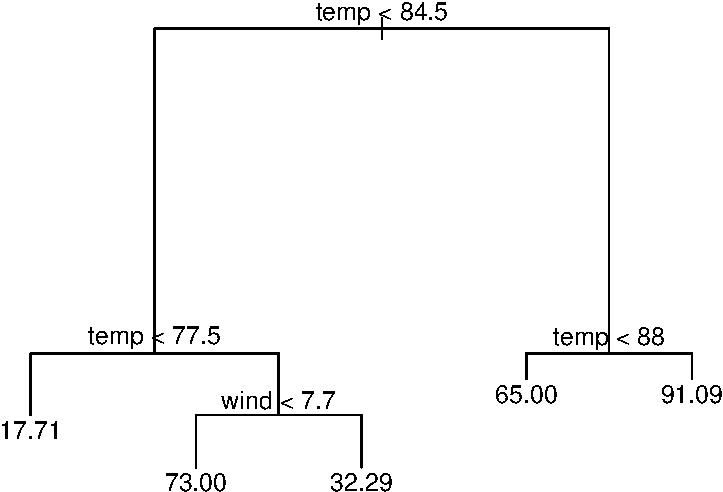
\includegraphics{RecEx7-sol_files/figure-latex/unnamed-chunk-7-1.pdf}

We see \texttt{displacement} has two peaks, \texttt{horsepower} has the
smallest CI for low values, the linear function in \texttt{weight} is
very variable for small and high values, \texttt{acceleration} looks
rather like a cubic function and there is a clear effect of
\texttt{origin}.

\end{document}
